\section{Evaluation}\label{sec:evaluation}

We now evaluate the tightness, time complexity and output size of routing function and pipeline characterization numerically. All experiments are conducted on a 1.6 GHz Intel Core i5 with 4 GB RAM.

%We now evaluate the characterization of a routing function and a pipeline from the tightness, computation complexity, and output size.  and running OS X system.

\subsection{Routing Function Characterization Tightness}
\label{sec:eval1}

We demonstrate the tightness of our characterization of a routing function by comparing the number of equivalence classes of a $M$ for both $\tau$ and $\tau_G$ for the following set of simple routing functions:

%We have examined the tightness of characterization of a routing function by comparing the $ec(M)$, the number of equivalent classes for a set of matches $M$, from two mappings (\ie, $\tau$ and $\tau_G$) for several routing functions. The computation of $ec(M)$ for the mapping $\tau$ is based on the definition of f-equivalence which will get the exact value of the number of equivalent classes of a set of matches $M$ for a particular routing function. The routing functions we use are shown as follows :

{\small
\begin{verbatim}
\\  Routing function: simpleRoute
L0: def simpleRoute(Addr srcIP, Addr dstIP):
L1:   srcSw = hostTbl[srcIP]
L2:   dstSw = hostTbl[dstIP]
L3:   route = routeTbl[srcSw, dstSw]
L4:   return route
\end{verbatim}
}

Our first function, \texttt{simpleRoute} maps a packet's \texttt{srcIP} and \texttt{dstIP} to their host packet switches \texttt{dstSw} and \texttt{srcSw} and then looks up the route between them.

%Function 1 (\texttt{simpleRoute}) reads two inputs and maps them to internal variables respectively based on a table, \texttt{hostTbl}. After that, \texttt{simpleRoute} gets the route from another table, \texttt{routeTbl}, where the key is two internal variables.

{\small
\begin{verbatim}
//  Routing Function: condRoute
L0: condRoute(srcIP, dstIP):
L1:   srcSw = hostTbl[srcIP]
L2:   dstSw = hostTbl[dstIP]
L3:   routeCond = condTbl[srcIP, dstIP]
L4:   route = routeTbl[srcSw, dstSw, routeCond]
L5:   return route
\end{verbatim}
}
Our second function \texttt{condRoute} extends \texttt{simpleRoute} by introducing a route condition variable which modulates the function's route look up.

%Function 2 (\texttt{f2}) is similar to \texttt{simpleRoute} except that there is a third table, \texttt{condTbl}, which returns an internal variable, \texttt{cond}, used as a part of the key of \texttt{routeTbl}.

{\small
\begin{verbatim}
//  Routing Function: secureRoute
L0: secureRoute(Addr srcIP, Addr dstIP):
L1:   if (isFiltered(srcIP)):
L2:     return Drop()
L3:   else:
L4:     route = fwdTbl[dstIP]
L5:     return route
\end{verbatim}
}
Our final function \texttt{secureRoute} drops all traffic from \texttt{srcIP}s on a filter list and forwards remaining traffic.

\para{Results:} We present our results in Table~\ref{table:table1}. Specifically, in Table~\ref{table:table1}, column 2 defines the domain of \texttt{srcIP}, \texttt{dstIP}, columns 3-6 give the output ranges $O(tbls)$ of each table, and columns 7-10 give the values of selected fields in each function's $\tau(f)$ and $\tau_G(f)$. 

Note that the row b1(scR) and b2(scR) represent the two branches of \texttt{secureRoute}. We record N/A when a value is not applicable to a given function, and null for values of $\tau(f)$ where computation failed to halt.

%gives the characterization results for the four functions, \texttt{simpleRoute}, \texttt{f2}, \texttt{f3}, and \texttt{onPkt}. The second column, $bits(input)$, defines the number of bits of both inputs, \ie, \texttt{srcIP}, \texttt{dstIP}; We use $\#O(t)$ to represent the number of possible output value for the table $t$; We only evaluate the equivalent class value in the output vector of characterization of a function for a particular input; The notation $b1(\texttt{f3})$ represents the branch 1 in \texttt{f3}, \ie, L1$\to$L2, while $b2(\texttt{f3})$ represents the branch 2 in \texttt{f3}, \ie, L1$\to$L3$\to$L4$\to$L5.

In our evaluation of \texttt{simpleRoute} and \texttt{condRoute}, the results of $\tau$ and $\tau_G$ are almost identical in every case barring an extreme one where $O(\texttt{condTbl})$ = 1. Notably, our values of $\tau(f)$ and $\tau_G(f)$ are not influenced by the range of $routeTbl$ $O(\texttt{routeTbl})$. This implies there is no pattern between the allocation of routes to (\texttt{srcIP}, \texttt{dstIP}) pairs $\tau(f)$ can exploit to reduce its number of equivalence classes.

%From the evaluation of simpleRoute and f2, we can see the result of $\tau$ and $\tau_G$ are almost the same except an extreme case where $\#O(\texttt{condTbl})$ = 1. Also, the results are not influenced by $\#O(\texttt{routeTbl})$, which can be observed from the first three rows in the table. This is because, considering $s_1$ and $s_2$ as two values of $srcIP$, if \texttt{hostTbl}($s_1$) is not equal to \texttt{hostTbl}($s_2$), then the chance of $s_1 \sim_f s_2$ is very small.

Further notice that our functions with control statements: \texttt{secureRoute} and \texttt{onPkt} have a large gap between $\tau$ and $\tau_G$, suggesting $\tau_G$'s bound is loose on heavily branching programs. However, as rows b1(scR) and b2(scR) show, we can ameliorate this problem  by calculating each route through a program characteristic function separately. 

%For the functions with control statements, such as f3, the results of $\tau$ and $\tau_G$ have a large gap. However, in this case, we can split the function into different branches. For each branch, the result of $\tau$ and $\tau_G$ maintains the tightness, which is shown in the rows with $b1(\texttt{f3})$ and $b2(\texttt{f3})$ in Table~\ref{table:table1}. Also, we evaluate the example routing function \texttt{onPkt}, and the result is shown in the last row in the table. Need to mention that, both $\tau$(f)(\texttt{srcIP}) and $\tau$(f)(\texttt{dstIP}) are null means that the computation time is too long to compute the result.

\begin{table*}[t]
\centering
\scalebox{0.75}{
\begin{tabular}{ | l | l | l | l | l | l | l | l | l | l | }
    \hline
    $f$ & $bits(IP)$ & $O(\texttt{hostTbl})$ & $O(\texttt{routeTbl})$ & $O(\texttt{condTbl})$ & $O(\texttt{fwdTbl})$ & $\tau$(f)(\texttt{srcIP}) & $\tau$(f)(\texttt{dstIP}) & $\tau_G$(f)(\texttt{srcIP}) & $\tau_G$(f)(\texttt{dstIP}) \\
    \hline   
    smplR & 10 & 100 & 2 & N/A & N/A  & 100 & 100 & 100 & 100 \\
    smplR & 10 & 100 & 30 & N/A & N/A & 100 & 100 & 100 & 100 \\
    smplR & 10 & 100 & 5000 & N/A & N/A & 100 & 100 & 100 & 100 \\
    smplR & 12 & 100 & 30 & N/A & N/A & 100 & 100 & 100 & 100 \\
    smplR & 10 & 200 & 30 & N/A & N/A & 200 & 200 & 200 & 200 \\
    condR & 10 & 100 & 30 & 50 & N/A & 1024 & 1024 & 1024 & 1024 \\
    condR & 10 & 100 & 30 & 5 & N/A & 1024 & 1024 & 1024 & 1024 \\
    condR & 10 & 100 & 30 & 1 & N/A & 100 & 100 & 1024 & 1024 \\
    scR & 10 & N/A & N/A & N/A & 100 & 2 & 100 & 2 & 1024 \\
    b1(scR) & 10 & N/A & N/A & N/A & N/A & 1 & N/A & 1 & N/A \\
    b2(scR) & 10 & N/A & N/A & N/A & 100 & 1 & 100 & 1 & 100 \\
    \texttt{onPkt} & 32 & 100 & 30 & 50 & N/A & null & null & $2^{32}$ & $2^{32}$ \\
    \hline
  \end{tabular}
  }
\vspace{1mm}
\caption{Characterization results of routing functions with different statistics.}
\label{table:table1}
\end{table*}


\subsection{Routing Function Characterization Time Complexity}
We now compare the time required to compute $\tau$ and $\tau_G$ for given routing functions. We run our tests using \texttt{simpleRoute} where $O(\texttt{hostTbl})$ = 100 and $O(\texttt{routeTbl})$ = 30.

%We have examined the computing complexity of characterization of a routing function by comparing the computation time of two mappings (\ie, $\tau$ and $\tau_G$) for the same function. As the same with the first evaluation, the computation of $\tau$ is based on the definition of f-equivalence. We use \texttt{Function 1} as a target function with fixed table entries where $O(\texttt{hostTbl})$ = 100 and $O(\texttt{routeTbl})$ = 30 to do the evaluation.

\para{Results:} Fig.~\ref{fig:e2-figure} shows the scalability of $\tau_G$ as input length grows. As \texttt{srcIP} and \texttt{dstIP}) bit length increase, $\tau_G$'s computation time remains constant while $\tau$'s computation time grows rapidly.

%$the computation time of $\tau_G$ has no change compared with the computation time of $\tau$ which grows rapidly.

%it requires large computation time based on the definition of f-equivalence to compute $\tau$ when the number of bits is large, while the computation of $\tau_G$ can be scalable with the number of bits of inputs (\ie, srcIP, dstIP) growing.

\begin{figure}[tbh]
    \centering
    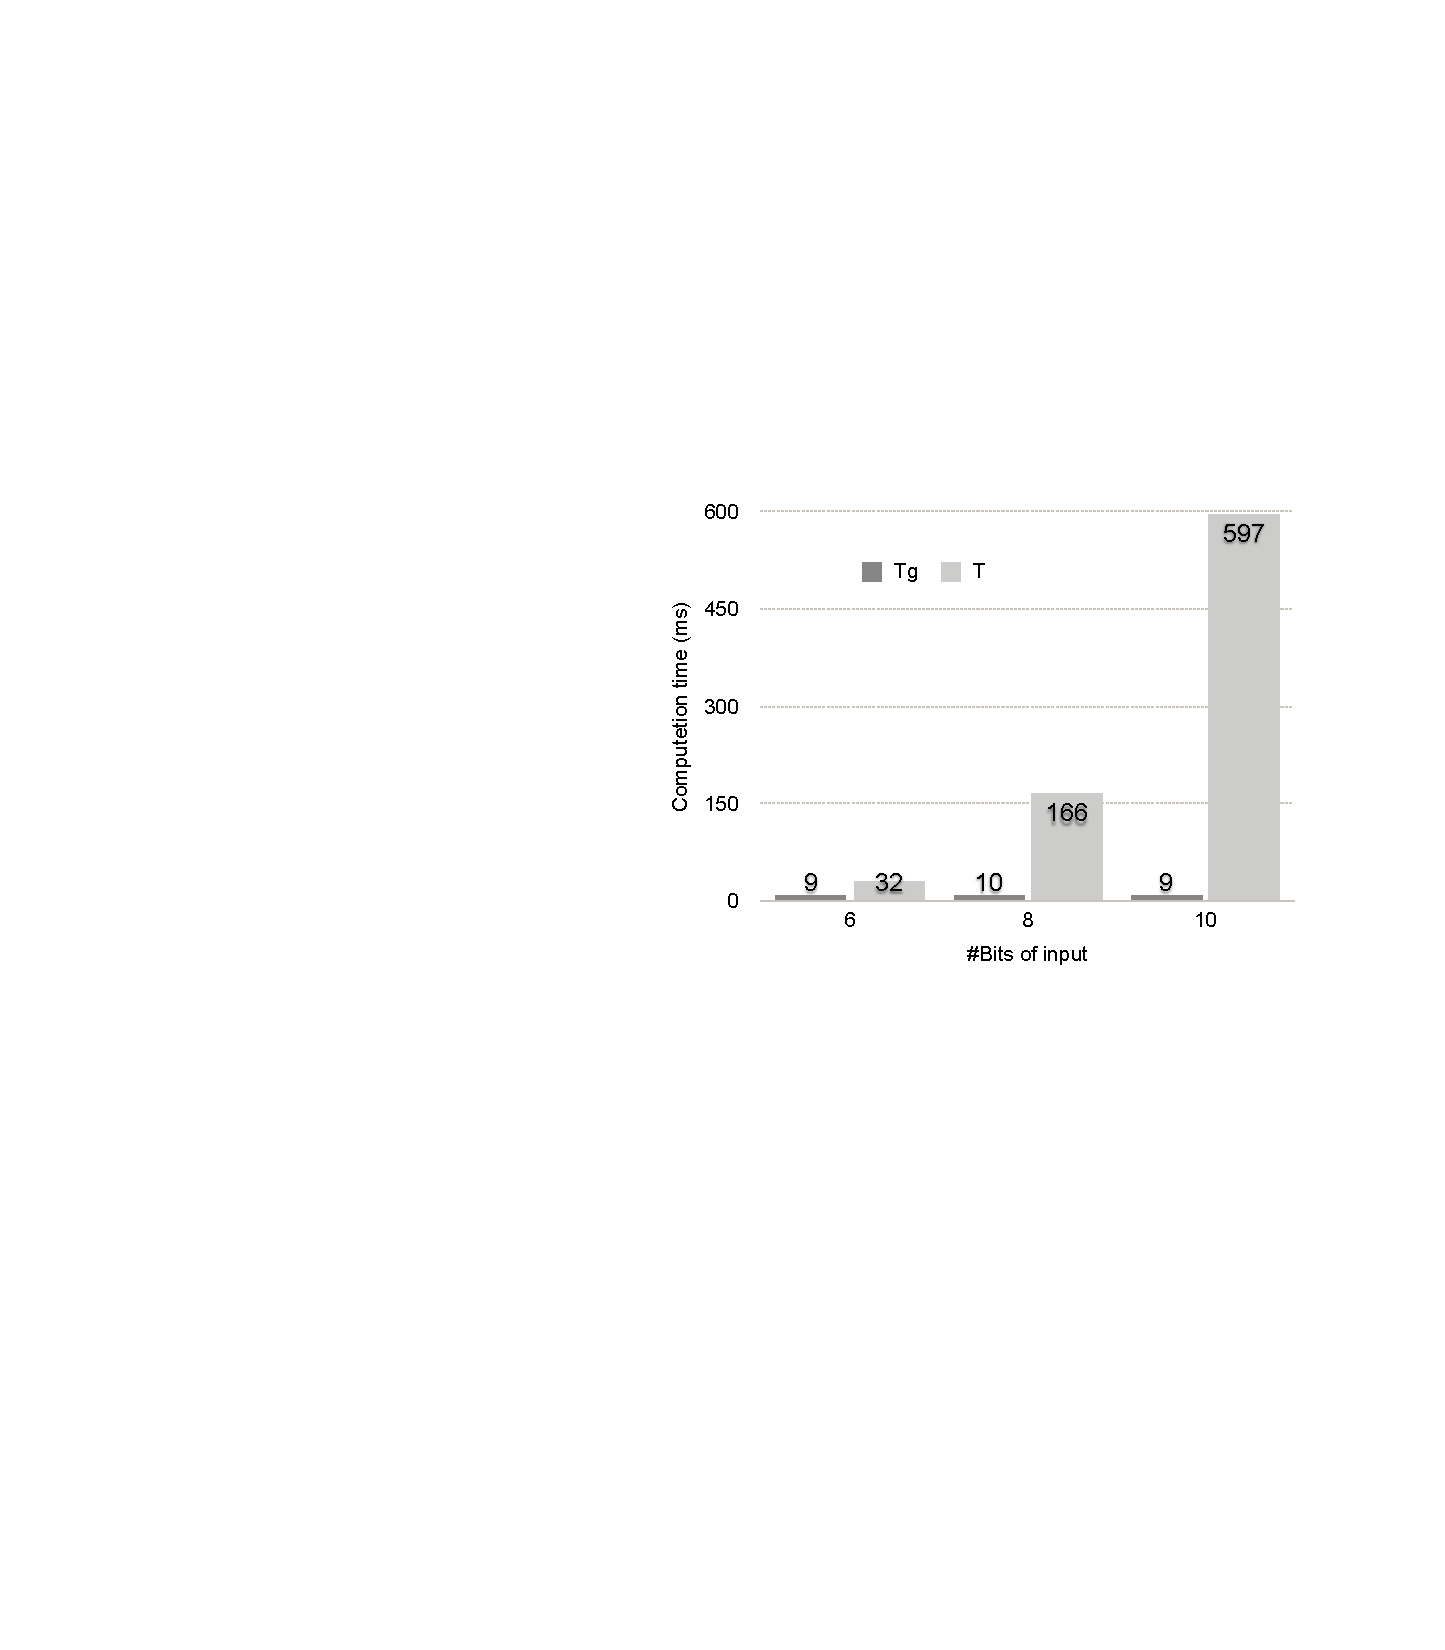
\includegraphics[scale = 0.6]{figures/e2-figure.pdf}
\vspace{-3mm}
    \caption{Computation time required to generate $\tau(\texttt{simpleRoute})$ and $\tau_G(\texttt{simpleRoute})$ as input bit length varies.}
    \label{fig:e2-figure}
\end{figure}

\subsection{Characterization of a Pipeline}

We now examine the memory utilization and computation time of pipeline characterization. We evaluate the following pipelines:

%We have examined the characterization of a pipeline by evaluating the computation time and compactness of characterization functions of several pipelines. The compactness of a characterization function of a pipeline represents the output memory utilization of the characterization function compared with the size of all the possible $M$. We use the following pipelines in the evaluation:

\begin{enumerate}
  \item \textbf{The OF-DPA Abstract Switch 2.0:} The OpenFlow Data Plane Abstraction Abstract Switch 2.0 (OF-DPA) is an abstract switch model based on the Open Flow 1.3.4 protocol designed to allow the programming of Broadcom-based switches under the OpenFlow protocol. We examine two OF-DPA flow table configurations: bridging and routing (BR), and data center overlay tunnel (OT), which contain 7, and 3 tables in 5, 3 stages respectively.~\cite{OF-DPA}

  \item \textbf{PicOS:} PicOS is a network operating system for white box switches that provides OF programmability across HP, Edgecore and Pica switches. We examine two fixed pipelines offered by PicOS as table type patterns: PicOS's IP routing pipeline (IPR) and Policy routing pipeline (PR), which contain 4 and 5 tables in 4 and 5 stages respectively.~\cite{PicOS}
\end{enumerate}

\para{Results:} Table~\ref{tbl:table3} our characterization results for our evaluated pipelines. The results show that despite the theoretically large number of subsets of $\mathcal{M}$ across evaluated pipelines, memory utilization and computation time are small.


%shows the characterization results of several pipelines including four real pipeline structures and the example pipeline, \exampledp. We say a set of packet match fields $M$ is valid in a pipeline $p$ means the value of $\kappa_\rho(\rho)(M)$ can be computed by the first formula in the definition of $\kappa_\rho(\rho)(M)$.  The result shows that though there are many combinations of $M$ for the output of characterization of a pipeline, the real memory utilization should be small. Also, it shows the computation of pipeline characterization is very fast.

\begin{table}[t]
\scalebox{0.8}{
\begin{tabular}{ | l | l | l | l | l | }
    \hline
    Pipeline & \#Paths & Time (ms) & \#Valid $M$ & \#$M$ \\
    \hline
    \exampledp & 3 & 8 & 6 & 22 \\
    PicOS BR & 4 & 13 & 19 & $3*(2^{24})+2^7$ \\
    PicOS OT & 2 & 7 & 5 & $2^{24} + 16$ \\
    Broadcom IPR & 1 & 7 & 4 & $2^7$ \\
    Broadcom PR & 3 & 9 & 14 & $2*(2^{24})+2^7$ \\
    \hline
  \end{tabular}
  }

\vspace{2mm}
\caption{Characterization results of pipelines.}
\label{tbl:table3}
\end{table}

%
%The goal of our evaluation is to demonstrate that the pipeline capacity theorem allows us to determine whether a generic program can be compiled to a fixed pipeline in a memory and time efficient manner for state-of-the-art programs and hardware. We then discuss a range of usage scenarios that our theorem enables. %All experiments are conducted on a processor Intel Core i5 running at 1.6 GHz, with 4 GB RAM and running OS X system. 
%
%\subsection{Setup, Pipelines and Programs}
%All experiments are conducted on a single processor 10-core (20-virtual thread) Intel(R) Xeon(R) CPU E5-2650 v3 machine running at 2.3 GHz, with 64GB RAM and running 64 bit Fedora Linux 24.
%
%
%\para{Pipelines:} We use the following pipelines in our experiments.
%
%\begin{enumerate}
%  \item \textbf{The OF-DPA Abstract Switch 2.0:} The OpenFlow Data Plane Abstraction Abstract Switch 2.0 (OF-DPA) is an abstract switch model based on the Open Flow 1.3.4 protocol designed to allow the programming of Broadcom-based switches under the OpenFlow protocol. We examine 3 OF-DPA flow table configurations: bridging and routing, data center overlay tunnel, and VPWS, which contain 17, 9, and 15 tables in 8, 5, and 12 stages respectively.~\cite{OF-DPA}
%
%  \item \textbf{PicOS:} PicOS is a network operating system for white box switches that provides OF programmability across HP, Edgecore and Pica switches. We examine two fixed pipelines offered by PicOS as table type patterns: PicOS's IP routing pipeline and Policy routing pipeline, which contain 7 and 8 tables in 5 and 6 stages respectively.~\cite{PicOS}
%\end{enumerate}
%
%\para{Programs:} Further, we test the following programs in our experiments:
%
%\begin{enumerate}
%\item\textbf{Program 1:}
%\end{enumerate}
%
%\subsection{Capacity vector calculation}
%
%\subsection{Transmission vector calculation}
%
%\subsection{Capacity transmission vector comparison}
